\subsubsection{Software del servidor}
Para la visualización y representación de los distintos valores de tensión y corriente medidos por los diferentes sensores, se ha optado por utilizar ThingsBoard, una plataforma IoT de código abierto para la recopilación, el procesamiento, la visualización y la gestión de dispositivos de datos.

\begin{figure}[H]
    \centering
    
\includegraphics[width=0.3\textwidth]{images/3-software/3-2-2-thingsboard/LogoThingsboard.png}
    \caption{Plataforma ThingsBoard}
    \label{fig:3-2-2-ThingsBoard}
\end{figure}

Para su instalación en el ordenador, se ha optado utilizar una máquina virtual en VirtualBox mediante la imagen de un servidor Linux con distribución Ubuntu. Para la realización de dicha instalación se ha seguido la guía oficial de la plataforma de ThingsBoard, que se puede definir en los siguientes pasos:
\todo[inline]{citar GUIA INSTALACION THINGSBAORD}

\begin{enumerate}
    \item Instalar Java17 y configurarlo como predeterminado mediante los comandos:
    \begin{verbatim}
sudo apt update
sudo apt install openjdk-17-jdk
sudo update-alternatives --config java
    \end{verbatim}

    \item Instalar ThingsBoard mediante los siguientes comandos:
    \begin{verbatim}
wget https://github.com/thingsboard/thingsboard/releases/download/v3.8.1/thingsboard-3.8.1.deb
sudo dpkg -i thingsboard-3.8.1.deb
    \end{verbatim}

    \item Configurar la base de datos de ThingsBoard:
    \begin{verbatim}
sudo apt install -y postgresql-common
sudo /usr/share/postgresql-common/pgdg/apt.postgresql.org.sh
sudo apt -y install postgresql-16
sudo service postgresql start
sudo su - postgres
psql
    \end{verbatim}
    A continuación, elige tu contraseña del postgres mediante el siguiente comando:
    \begin{verbatim}
\password
    \end{verbatim}
    Después pulsa ``Ctrl + D'' para volver atrás y utiliza el siguiente comando para conectarte a la base de datos postgres:
    \begin{verbatim}
psql -U postgres -d postgres -h 127.0.0.1 -W
    \end{verbatim}
    Ahora, crea la base de datos para Thingsboard mediante el comando: \\
    \texttt{CREATE DATABASE thingsboard;} \\
    Por último, pulsa dos veces ``Ctrl + D'' para salir del PostgreSQL.

    \item Modificar el archivo de configuración de ThingsBoard mediante el siguiente comando:
    \begin{verbatim}
sudo nano /etc/thingsboard/conf/thingsboard.conf
    \end{verbatim}
    A continuación, añade estas líneas al final del archivo y no olvides cambiar \\
    \texttt{PUT\_YOUR\_POSTGRESQL\_PASSWORD\_HERE} por la contraseña del postgres que pusiste anteriormente:
    \begin{verbatim}
# DB Configuration
export DATABASE_TS_TYPE=sql
export SPRING_DATASOURCE_URL=jdbc:postgresql://localhost:5432/thingsboard
export SPRING_DATASOURCE_USERNAME=postgres
export SPRING_DATASOURCE_PASSWORD=PUT_YOUR_POSTGRESQL_PASSWORD_HERE
# Specify partitioning size for timestamp key-value storage.
# Allowed values: DAYS, MONTHS, YEARS, INDEFINITE.
export SQL_POSTGRES_TS_KV_PARTITIONING=MONTHS
    \end{verbatim}

    \item Elegir el tipo de servicio de cola de ThingsBoard. En este caso se elige el por defecto, en memoria, por lo que no es necesario ningún paso adicional.

    \item Ejecutar el script de instalación mediante el siguiente comando:
    \begin{verbatim}
sudo /usr/share/thingsboard/bin/install/install.sh --loadDemo
    \end{verbatim}

    \item Arrancar el servicio de ThingsBoard mediante el siguiente comando:
    \begin{verbatim}
sudo service thingsboard start
    \end{verbatim}
\end{enumerate}

Una vez realizados estos pasos, se podrá acceder a ThingsBoard mediante el siguiente link: \\
\url{http://localhost:8080/}

Por defecto, ThingsBoard incluye tres diferentes perfiles para acceder a la plataforma:
\begin{itemize}
    \item System Administrator: \texttt{sysadmin@thingsboard.org / sysadmin}
    \item Tenant Administrator: \texttt{tenant@thingsboard.org / tenant}
    \item Customer User: \texttt{customer@thingsboard.org / customer}
\end{itemize}

Debido al uso de la máquina virtual, se ha tenido que realizar una redirección de los puertos mediante la interfaz de red de la propia máquina, obteniendo la siguiente configuración:

\begin{figure}[H]
    \centering
    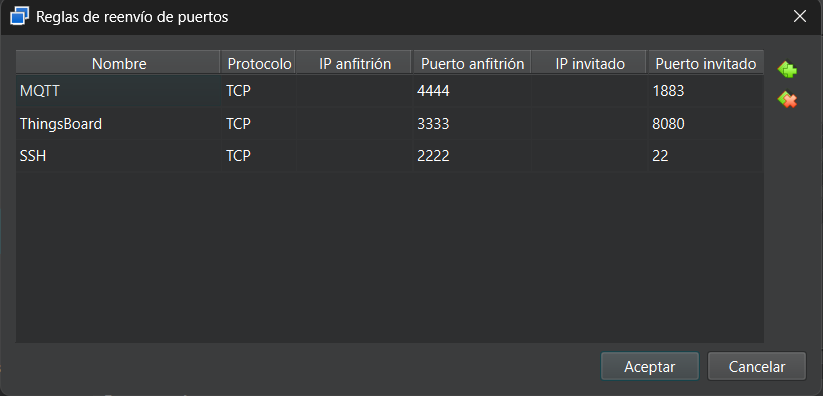
\includegraphics[width=0.3\textwidth]{images/3-software/3-2-2-thingsboard/PuertosMV.png}
    \caption{Redirección de puertos MV}
    \label{fig:3-2-2-PuertosMV}
\end{figure}

Por lo que, en nuestro caso, el puerto 1883 correspondiente al MQTT broker se corresponde con el puerto 4444 de la máquina virtual, el puerto 3333 de la plataforma ThingsBoard se corresponde con el puerto 8080 de la MV y también se ha redirigido el puerto 22 de SSH al puerto 2222 de la máquina virtual por conflictos internos con otro programa.

Para la comunicación entre la plataforma ThingsBoard y el dispositivo ESP8266, se ha implementado el broker Mosquitto, el cual es un broker MQTT OpenSource ampliamente utilizado debido a su ligereza, lo que permite fácilmente emplearlo en gran número de ambientes, incluso si éstos son de pocos recursos. A continuación se indica el comando necesario para su instalación, obtenido de la guía oficial de ThingsBoard:
\todo[inline]{Citar GUIA INSTALACION MQTT BROKER}
\begin{verbatim}
sudo apt-get install mosquitto-clients
\end{verbatim}

Para comprobar que todo se ha realizado correctamente, se puede utilizar el siguiente comando:
\begin{verbatim}
mosquitto_pub -d -q 1 -h "$THINGSBOARD_HOST_NAME" -p "1883"
-t "v1/devices/me/telemetry" -u "$ACCESS_TOKEN" -m {"ATTRIBUTE":25}
\end{verbatim}

Donde los siguientes parámetros corresponden con:
\begin{itemize}
    \item \texttt{THINGSBOARD\_HOST\_NAME}: dirección IP del servidor ThingsBoard, \\
    por ejemplo, \texttt{localhost} o \texttt{127.0.0.1}.
    \item \texttt{ACCESS\_TOKEN}: token de acceso único proporcionado por ThingsBoard para cada dispositivo.
    \item \texttt{ATTRIBUTE}: atributo asociado a dicho dispositivo, por ejemplo, temperature.
\end{itemize}

En caso de que la conexión y publicación se haya realizado de manera correcta, se obtendrá la siguiente respuesta:
\begin{verbatim}
Client mosqpub|xxx sending CONNECT
Client mosqpub|xxx received CONNACK
Client mosqpub|xxx sending PUBLISH
(d0, q1, r0, m1, 'v1/devices/me/telemetry', ... (16 bytes))
Client mosqpub|xxx received PUBACK (Mid: 1)
Client mosqpub|xxx sending DISCONNECT
\end{verbatim}

Una vez que se ha comprobado el correcto funcionamiento de la conexión entre la plataforma Thingsboard y el broker y cliente MQTT, se puede continuar con la personalización de dicha plataforma.

Para la visualización de los datos recibido, se ha optado por diseñar dos paneles o \textit{Dashboards}, uno en representación en forma de tablas y otro en forma de gráficas. Ambos paneles se actualizan en tiempo real y cuentan con una tabla o gráfica para cada dispositivo, obtenido un total de 4 tablas y 4 gráficas. Además, en las gráficas se puede visualizar también la media de los últimos datos medidos.

\begin{figure}[H]
    \centering
    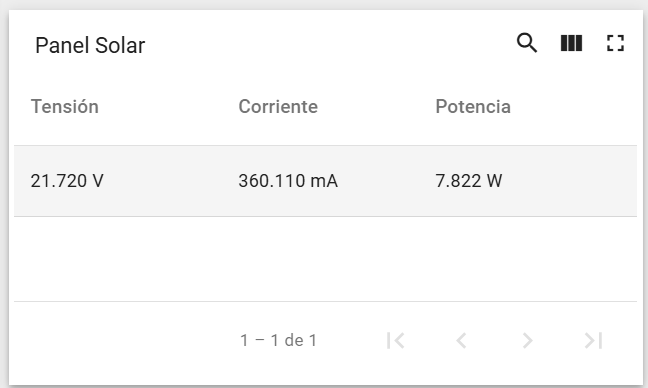
\includegraphics[width=0.3\textwidth]{images/3-software/3-2-2-thingsboard/TablaThingsBoard.png}
    \caption{Tabla de medidas}
    \label{fig:3-2-2-TablaThingsBoard}
\end{figure}

\begin{figure}[H]
    \centering
    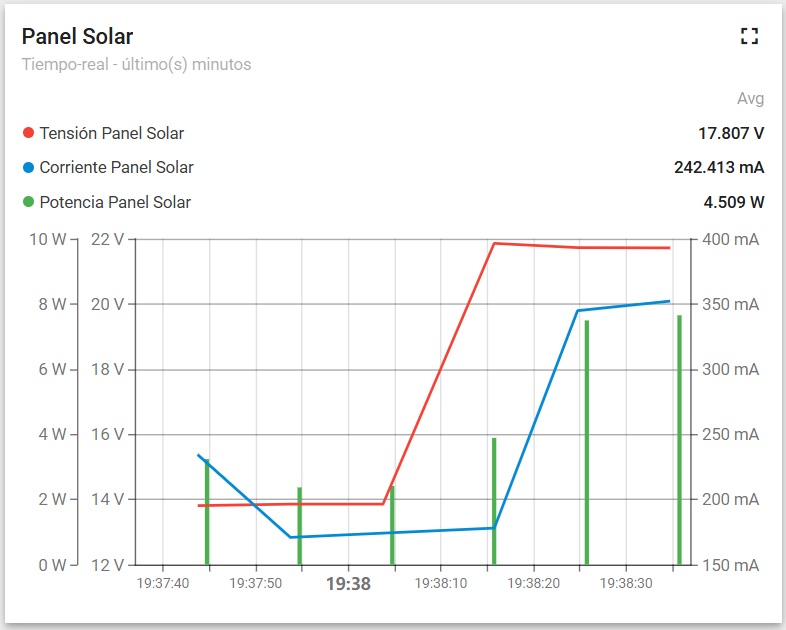
\includegraphics[width=0.3\textwidth]{images/3-software/3-2-2-thingsboard/GraficaThingsBoard.png}
    \caption{Gráfica de medidas}
    \label{fig:3-2-2-GraficaThingsBoard}
\end{figure}

Debido a que mediante los sensores solo se obtienen valores de tensión y de corriente, se ha implementado un algoritmo mediante las cadenas de reglas de Thingsboard. Se ha necesitado crear una cadena de reglas para cada potencia calculada, obteniendo 4 cadena de reglas como la siguiente:

\begin{figure}[H]
    \centering
    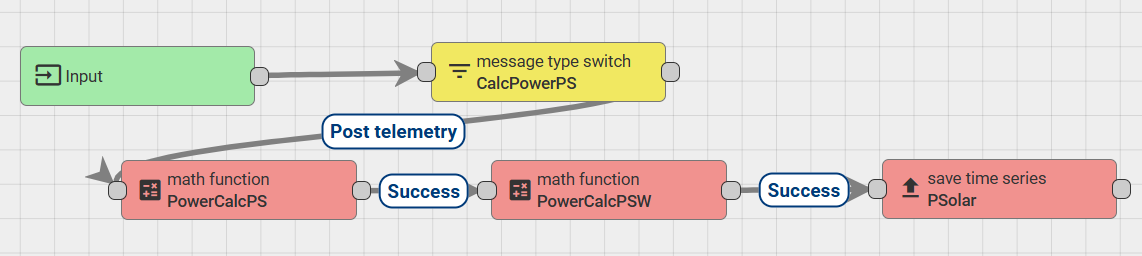
\includegraphics[width=0.3\textwidth]{images/3-software/3-2-2-thingsboard/CadenaPotencia.png}
    \caption{Cadena de reglas para cálculo de potencias}
    \label{fig:3-2-2-CadenaPotenciaThingsBoard}
\end{figure}

Dichas cadenas de reglas se dividen en los siguientes pasos:

\begin{enumerate}
    \item Filtrar y transformar la telemetría entrante
    \item Realizar el cálculo de la potencia correspondiente
    \item Pasar dicha potencia a Vatios
    \item Guardas los valores para su reprentación
\end{enumerate}

Por último, se ha añadido dichas cadenas de reglas de potencia a la cadena de regla principal, la cual gestiona el funcionamiento completo de Thingsboard y permite visualizar el dato obtenido de su respectiva cadena de regla.

\begin{figure}[H]
    \centering
    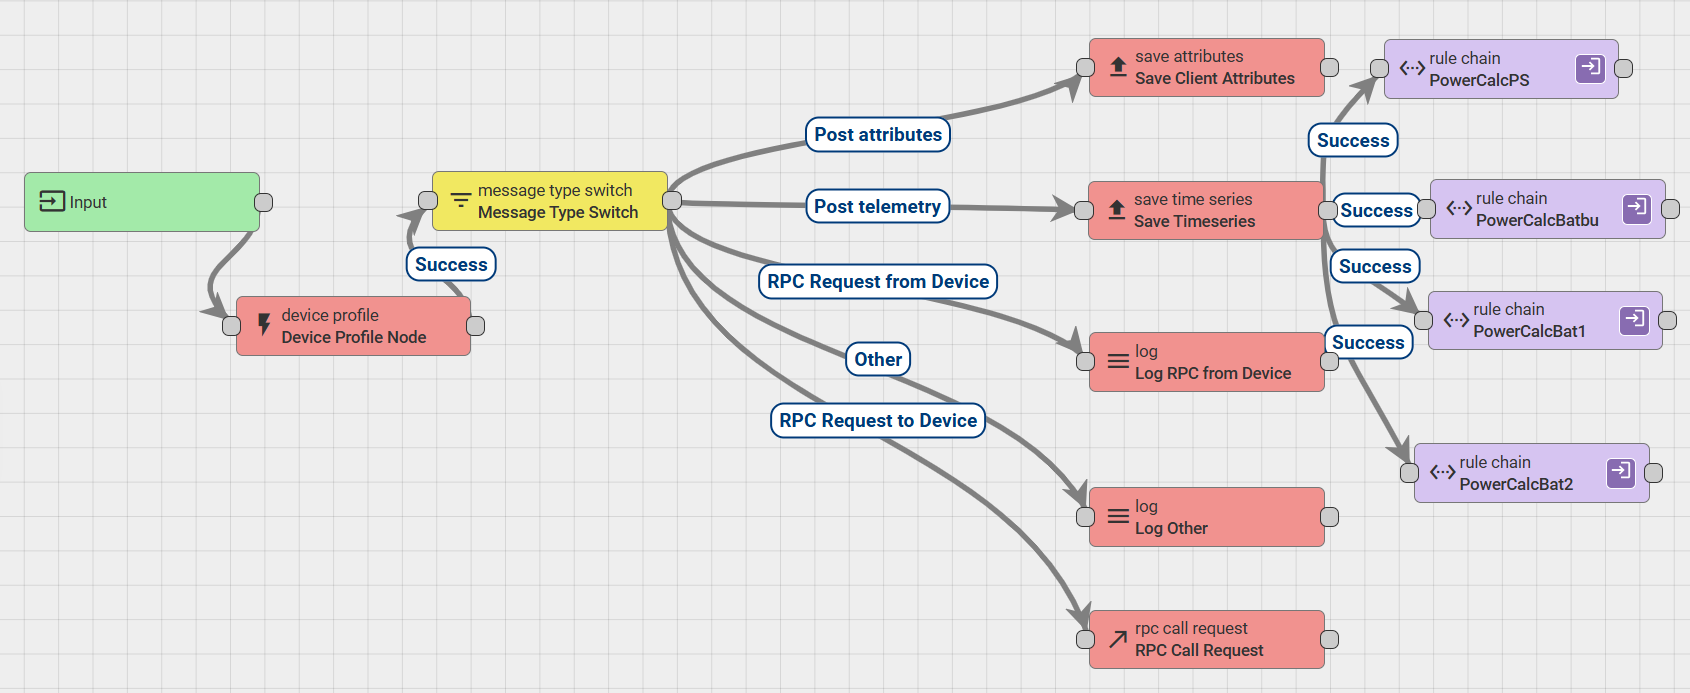
\includegraphics[width=0.3\textwidth]{images/3-software/3-2-2-thingsboard/CadenaPrincipal.png}
    \caption{Cadena de reglas principal}
    \label{fig:3-2-2-CadenaPrincipalThingsBoard}
\end{figure}